% pyformex manual --- examples
% $Id$
% (C) B.Verhegghe

\chapter{pyFormex example scripts}
\label{cha:examples}

\section{Creating geometry}
\label{sec:creating-geometry}

This section has not been written yet.

\section{Operating on surface meshes}
\label{sec:operating-surf-mesh}

Besides being used for creating geometries, \pyf also offers interesting possibilities for executing specialized operations on surface meshes, usually STL type triangulated meshes originating from medical scan (CT) images. Some of the algorithms developed were included in \pyf.

\subsection{Unroll stent}
\label{sec:unroll-stent}

A stent is a medical device used to reopen narrowed arteries. The vast majority of stents are balloon-expandable, which means that the metal structure is deployed by inflating a balloon, located inside the stent. Figure~\ref{fig:cypher-stent} shows an example of such a stent prior to expansion (balloon not shown). The 3D surface is obtained by micro CT and consists of triangles.

\begin{figure}[h]
  \centering
  \begin{makeimage}
  \end{makeimage}
  \begin{latexonly}
    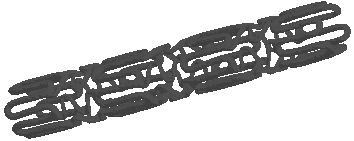
\includegraphics[width=8cm]{images/cypher-stent}
  \end{latexonly}
  \begin{htmlonly}
    \htmladdimg{../images/cypher-stent.png}
  \end{htmlonly}  
  \caption{Triangulated mesh of a stent}
  \label{fig:cypher-stent}
\end{figure}

The structure of such a device can be quite complex and difficult to analyse. The same functions \pyf offers for creating geometries can also be employed to investigate triangulated meshes. A simple unroll operation of the stent gives a much better overview of the complete geometrical structure and allows easier analysis (see figure~\ref{fig:cypher-stent-unroll}).
 
\code{F = F.toCylindrical().scale([1.,2*radius*pi/360,1.])}

\begin{figure}[h]
  \centering
  \begin{makeimage}
  \end{makeimage}
  \begin{latexonly}
    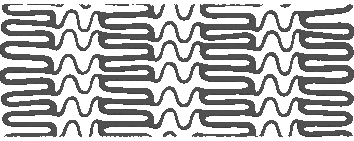
\includegraphics[width=8cm]{images/cypher-stent-unroll}
  \end{latexonly}
  \begin{htmlonly}
    \htmladdimg{../images/cypher-stent-unroll.png}
  \end{htmlonly}  
  \caption{Result of unroll operation}
  \label{fig:cypher-stent-unroll}
\end{figure}

This unrolled geometry can then be used for further investigations. An important property of such a stent is the circumference of a single stent cell. The \code{clip()} method can be used to isolate a single stent cell. In order to obtain a line describing the stent cell, the function \code{intersectionLinesWithPlane()} has been used. The result can be seen in figure~\ref{fig:stent-cell}.

\begin{figure}[h]
  \centering
  \begin{makeimage}
  \end{makeimage}
  \begin{latexonly}
    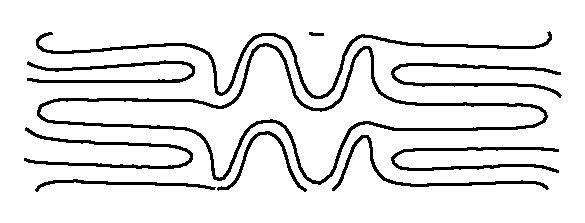
\includegraphics[width=6cm]{images/stent-cell-full}
  \end{latexonly}
  \begin{htmlonly}
    \htmladdimg{../images/stent-cell-full.png}
  \end{htmlonly}  
  \caption{Intersection of stent cell with plane}
  \label{fig:stent-cell-full}
\end{figure}


\begin{figure}[h]
  \centering
  \begin{makeimage}
  \end{makeimage}
  \begin{latexonly}
    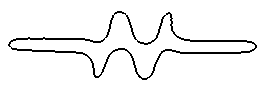
\includegraphics[width=6cm]{images/stent-cell}
  \end{latexonly}
  \begin{htmlonly}
    \htmladdimg{../images/stent-cell.png}
  \end{htmlonly}  
  \caption{Inner line of stent cell}
  \label{fig:stent-cell}
\end{figure}

Finally, the \code{length()} function returns the circumference of the cell, which is 9.19 mm.

%%% Local Variables: 
%%% mode: latex
%%% TeX-master: "manual"
%%% End: 
